\documentclass[twoside, final, 11pt]{articleMine}
\usepackage[english]{babel} \usepackage{a4wide}
\usepackage{amsmath,amssymb,accents} \usepackage{epsfig}
\usepackage{subfigure} \usepackage{units} \usepackage{graphicx}
\usepackage[displaymath, mathlines, right]{lineno} \usepackage{xspace}
\usepackage{color} \usepackage{epic,eepic,pstricks}
\usepackage{acronym} \usepackage{wrapfig,multicol}
\usepackage{deluxetable} \usepackage{todonotes} 
\usepackage{hyperref}
%\usepackage{slashbox}
\usepackage{lmodern} 
%\usepackage{caption}
\linenumbers
%\usepackage{showlabels}
\usepackage[draft]{showkeys}

%\usepackage[nolists, tablesfirst]{endfloat}
\graphicspath{{plots/}}
\newcommand*\patchAmsMathEnvironmentForLineno[1]{%
  \expandafter\let\csname old#1\expandafter\endcsname\csname #1\endcsname
  \expandafter\let\csname oldend#1\expandafter\endcsname\csname end#1\endcsname
  \renewenvironment{#1}%
     {\linenomath\csname old#1\endcsname}%
     {\csname oldend#1\endcsname\endlinenomath}}%
\newcommand*\patchBothAmsMathEnvironmentsForLineno[1]{%
  \patchAmsMathEnvironmentForLineno{#1}%
  \patchAmsMathEnvironmentForLineno{#1*}}%
\AtBeginDocument{%
\patchBothAmsMathEnvironmentsForLineno{equation}%
\patchBothAmsMathEnvironmentsForLineno{align}%
\patchBothAmsMathEnvironmentsForLineno{flalign}%
\patchBothAmsMathEnvironmentsForLineno{alignat}%
\patchBothAmsMathEnvironmentsForLineno{gather}%
\patchBothAmsMathEnvironmentsForLineno{multline}%
}
%\AtBeginFigures{\cleardoublepage}
%%%%%\parindent 5pt  
\parskip 1.2pt           % sets spacing between paragraphs
\def\Offline{\mbox{$\overline{\rm
Off}$\hspace{.05em}\raisebox{.4ex}{$\underline{\rm line}$}}\xspace}
\def\OfflineB{\mbox{$\bf\overline{\rm\bf
Off}$\hspace{.05em}\raisebox{.4ex}{$\bf\underline{\rm\bf line}$}}\xspace}

\def\eq#1{\begin{equation}#1\end{equation}}
%\def\al#1{\begin{align}#1\end{align}}
%\def\vc#1{{\bf #1}}
\def\pt#1{\accentset{\rightharpoonup}{#1}}
\include{myabbr}

\newcommand{\HRule}{\rule{\linewidth}{0.5mm}}
\newcommand{\VEM}{\mbox{VEM}}
\newcommand{\m}{\mbox{m}}

\let\stdsection\section  
%\renewcommand\section{\newpage\stdsection}  
 
\begin{document}

%\setpagewiselinenumbers
\modulolinenumbers[2]

%\linenumbers


\renewcommand\linenumberfont{\small\rmfamily}
\begin{center}
  \vspace*{-13ex}

  \rule{\linewidth}{0.1mm}  \\[17mm] {\huge  Detector simulation and validation with dat}
     \begin{flushright}
       \small 
     
     \end{flushright}

  % 
\end{center}
% 
\vspace*{2ex} 
%
\thispagestyle{empty}
\noindent
\begin{abstract}
  \noindent
We detail  in this note the  simulation method of  the EASIER detector
from the Radio Frequency (RF) signal to the ADC trace. We validate and
compare  our  models with  the  data  of  the three  different  C-band
detectors.
\end{abstract}

%
\thispagestyle{empty}
%$\;$
%\listoftodos
%\newpage
\noindent
%\section{Introduction}
The  current  signal  search for  EASIER  event  is  based on  a  peak
detection. To be  considered as an event, a peak  also needs to arrive
in coincidence with the trigger given by the particle signal and above
a fixed threshold.  It is robust  but it is not the best technique for
the search of small signals.  We study in this note the improvement of
the signal  to noise  ratio when  a matched filter  is applied  to the
radio trace.  %% This method can be applied to all type of EASIER
%% detectors  (EASIER/GD  C-band/GD helix).
\\ In  the first section  we present briefly the  detector simulations
needed  to   test  the   effect  of  the   filters.   Then   we  study
quantitatively    the   improvement    in   sensitivity    with   mock
signals. Finally, we apply these methods to realistic simulation data.

\section{Expected signal}
We present in this section the calculation of the expected signal. The
main ingredients are:
\begin{itemize}
\item the sun flux (the sun flux varies with time)
\item the sun path with respect to the antenna depending on the time of the year
\item the antenna pattern
\end{itemize}
Given these  ingredients can then  calculate the expected  increase of
power collected output by the antenna and deduce the expected increase
of the baseline for a given system temperature.

\subsection{Sun flux}
In our frequency range ~ GHz,  the sun flux has two main contributions
~\cite{solarflux}:  a quiet  sun component  (or  background component)
with a constant intensity and a frequency dependence as:
\begin{equation} 
 Sq \  [SFU] =  26.4 +  12.4 \ \nu  + 1.11\  \nu^2 \\ \rm  for \  (1 <
 \nu(GHz) < 20)
\end{equation}
a    second    contribution,   the    so    called   slowly    varying
component, its spectrum is parameterised as:
\begin{equation}
    Sv  \ [SFU]= \frac{0.64 ( F10.7 - 70 ) f^{0.4}}{ 1 + 1.56 ( ln \ ( \ f  \ / \  2.9 ) )^2}
\end{equation}
These spectra are shown in the figure~\ref{fig:spectra}
\begin{figure}[!ht]
  \centering
  \hspace*{-3ex}
  \subfigure{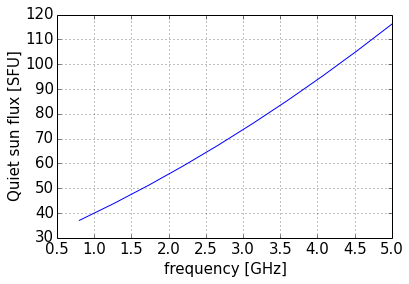
\includegraphics[width=0.49\linewidth]{quietsunspec.png}}
  \subfigure{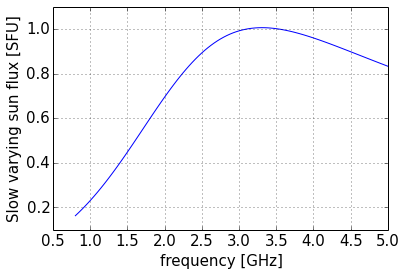
\includegraphics[width=0.49\linewidth]{varyingsunspec.png}}
  \caption{Left: quiet sun spectrum, Right: varying component spectrum}
  \label{fig:spectra}
\end{figure}
The  intensity of  the total  flux at  2.8GHz (F10.7)  is  measured by
several  observatories\cite{nobeyamaobs}, \cite{nasa}.  Making  use of
these data  and the parameterization  in frequency written  above, one
can deduce the flux in the C-band.


\paragraph{F10.7}
\begin{figure}[!ht]
  \centering
  \hspace*{-3ex}
  \subfigure{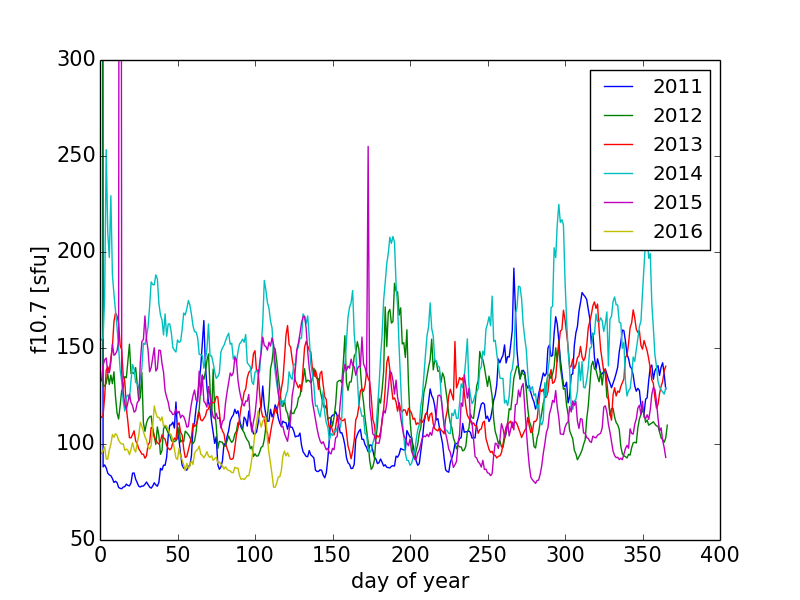
\includegraphics[width=0.7\linewidth]{f10_72011_2016.png}}
  \caption{Left: quiet sun spectrum, Right: varying component spectrum}
  \label{fig:spectra}
\end{figure}


\paragraph{sun path}
\begin{figure}[!ht]
  \centering
  \hspace*{-3ex}
  \subfigure{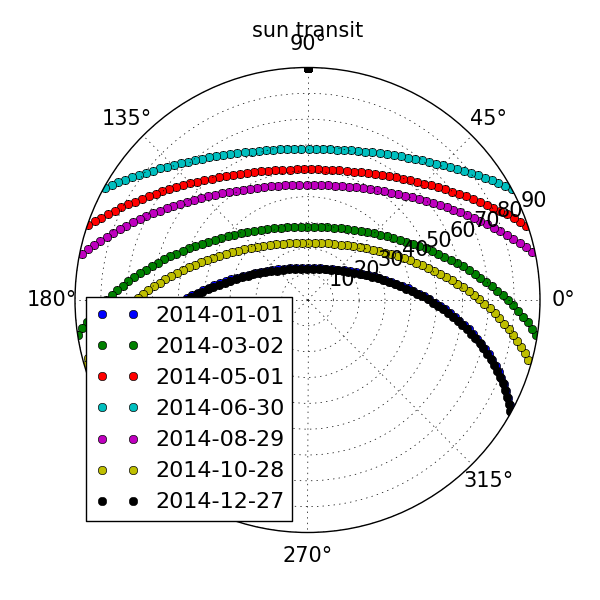
\includegraphics[width=0.7\linewidth]{sunpath.png}}
  \caption{Left: quiet sun spectrum, Right: varying component spectrum}
  \label{fig:spectra}
\end{figure}

\paragraph{expected signal}
\begin{figure}[!ht]
  \centering
  \hspace*{-3ex}
  \subfigure{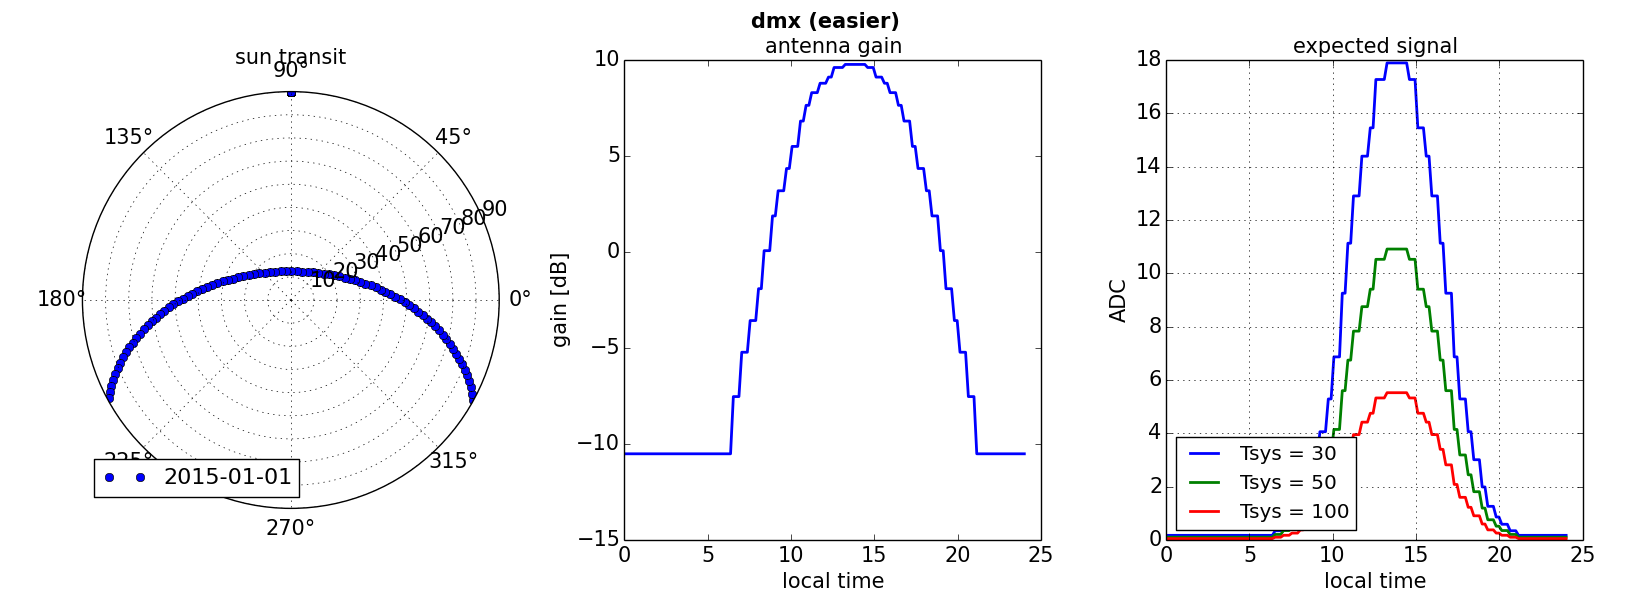
\includegraphics[width=0.7\linewidth]{expeasier.png}}\\
  \subfigure{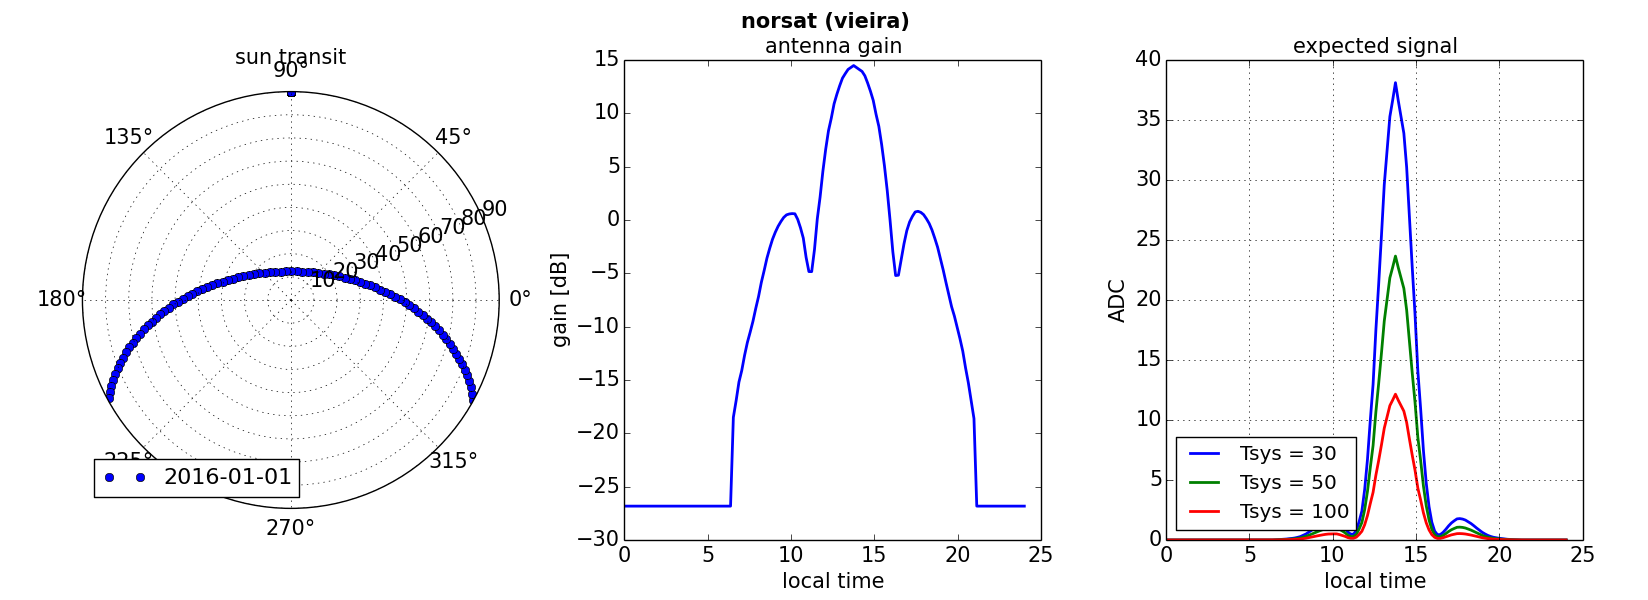
\includegraphics[width=0.7\linewidth]{expvieira20160101.png}}\\
  \subfigure{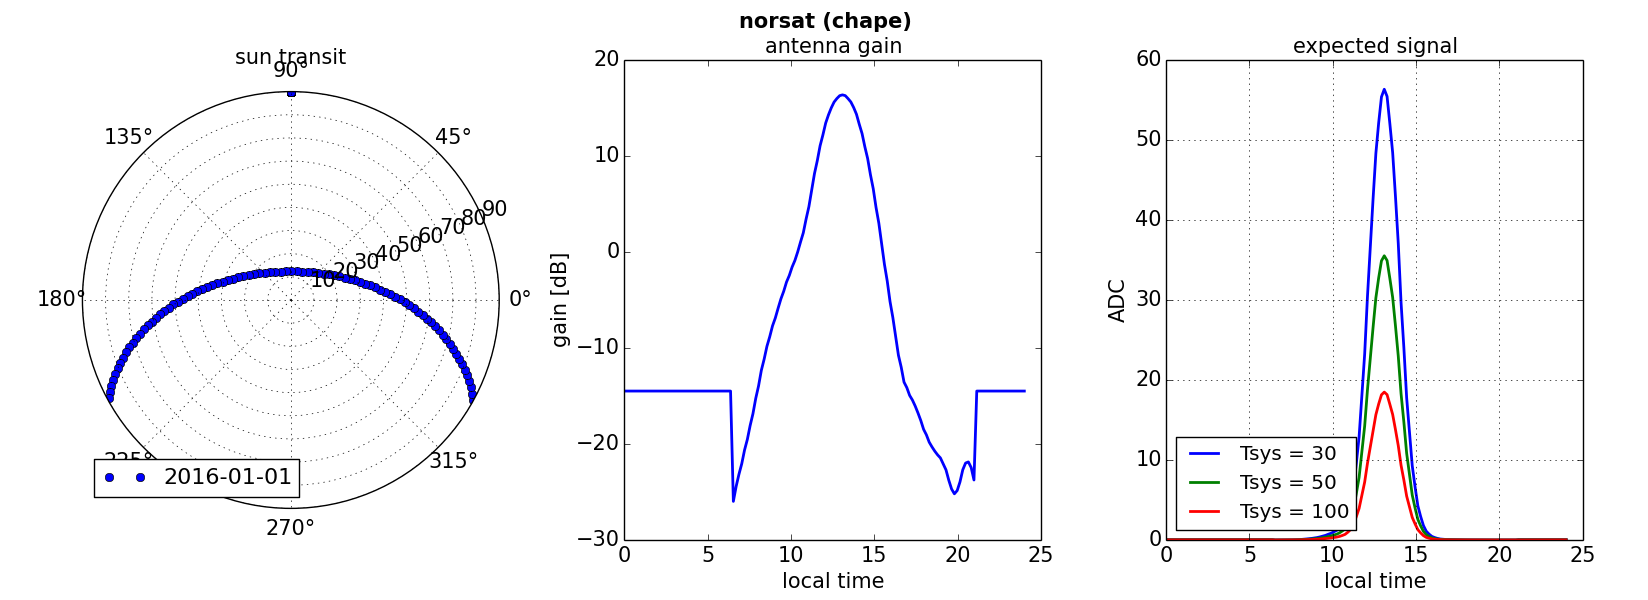
\includegraphics[width=0.7\linewidth]{expchape20160101.png}}\\
  \subfigure{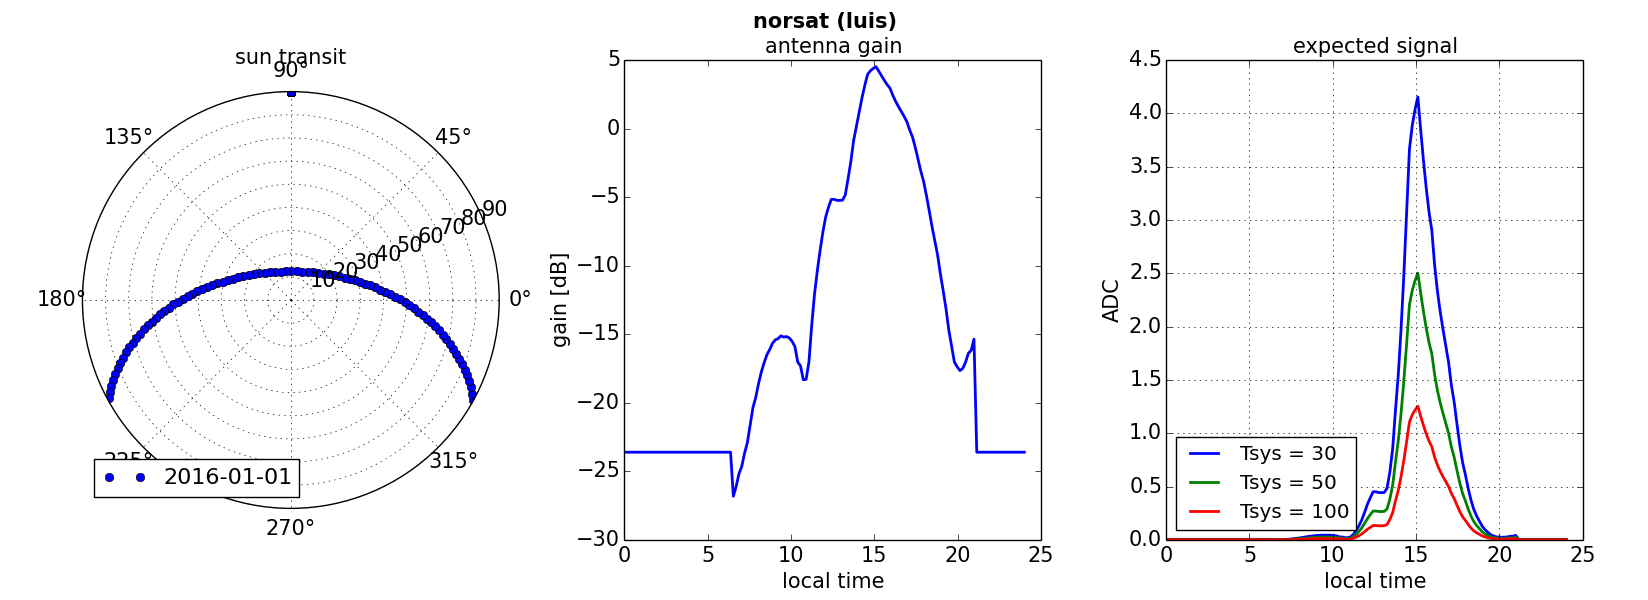
\includegraphics[width=0.7\linewidth]{expluis20160101.png}}\\
  \caption{Left: quiet sun spectrum, Right: varying component spectrum}
  \label{fig:spectra}
\end{figure}

\begin{figure}[!ht]
  \centering
  \hspace*{-3ex}
  \subfigure{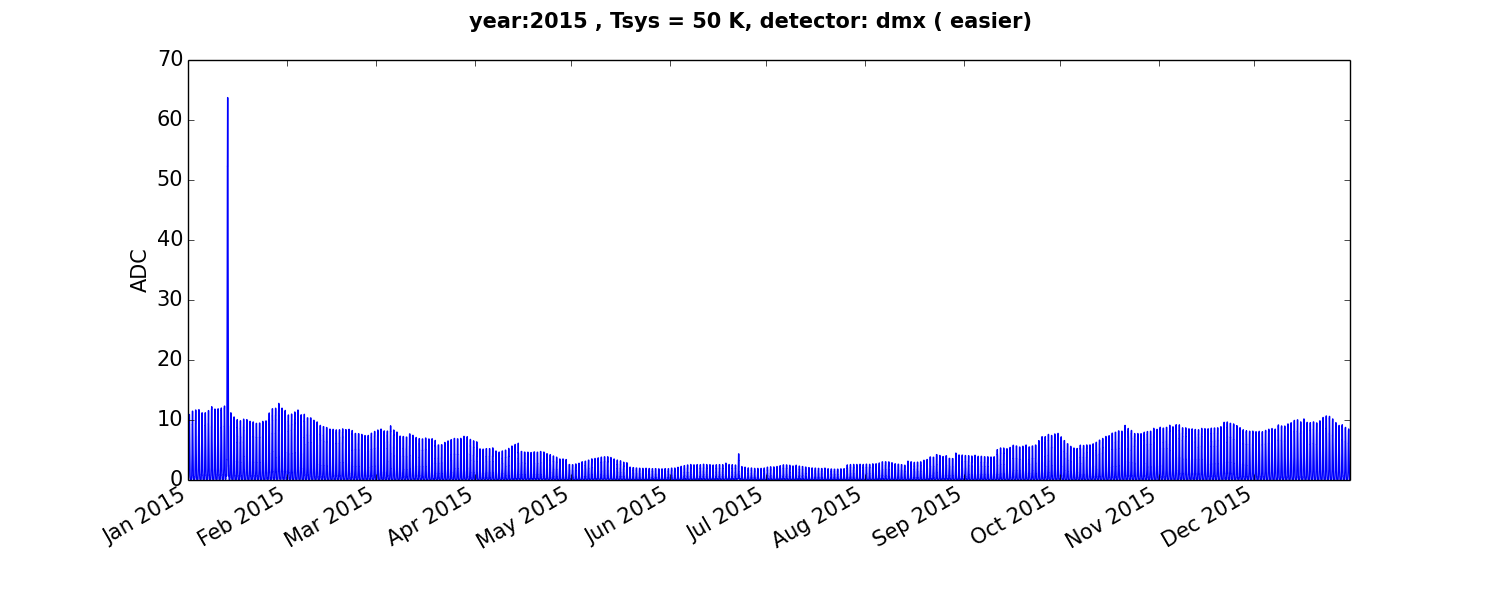
\includegraphics[width=0.7\linewidth]{year2015easier.png}}\\
  \subfigure{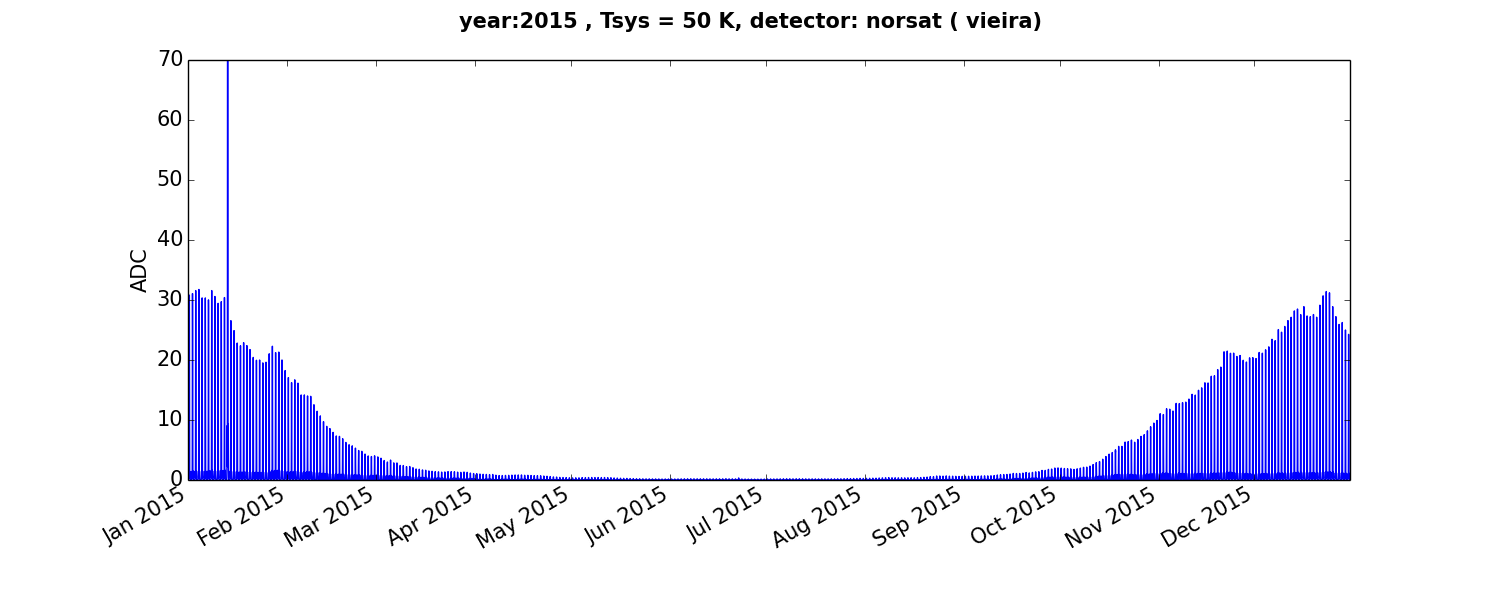
\includegraphics[width=0.7\linewidth]{year2015vieira.png}}\\
  \subfigure{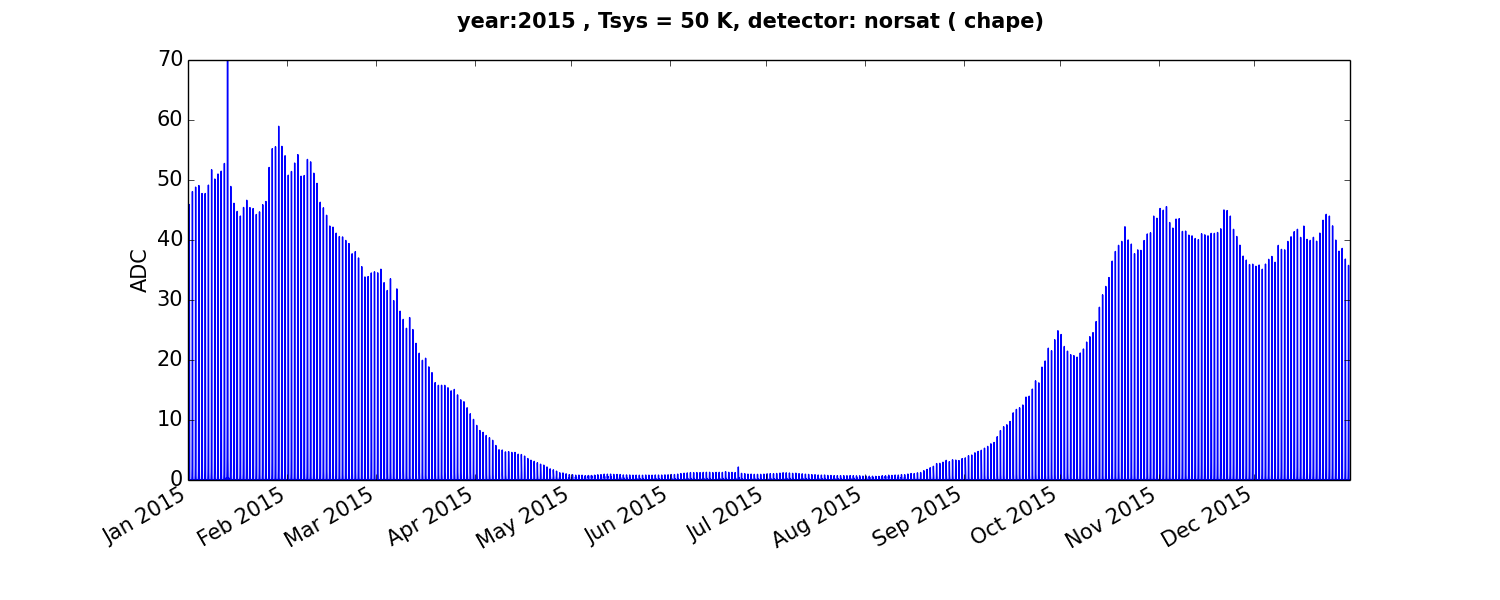
\includegraphics[width=0.7\linewidth]{year2015chape.png}}\\
  \subfigure{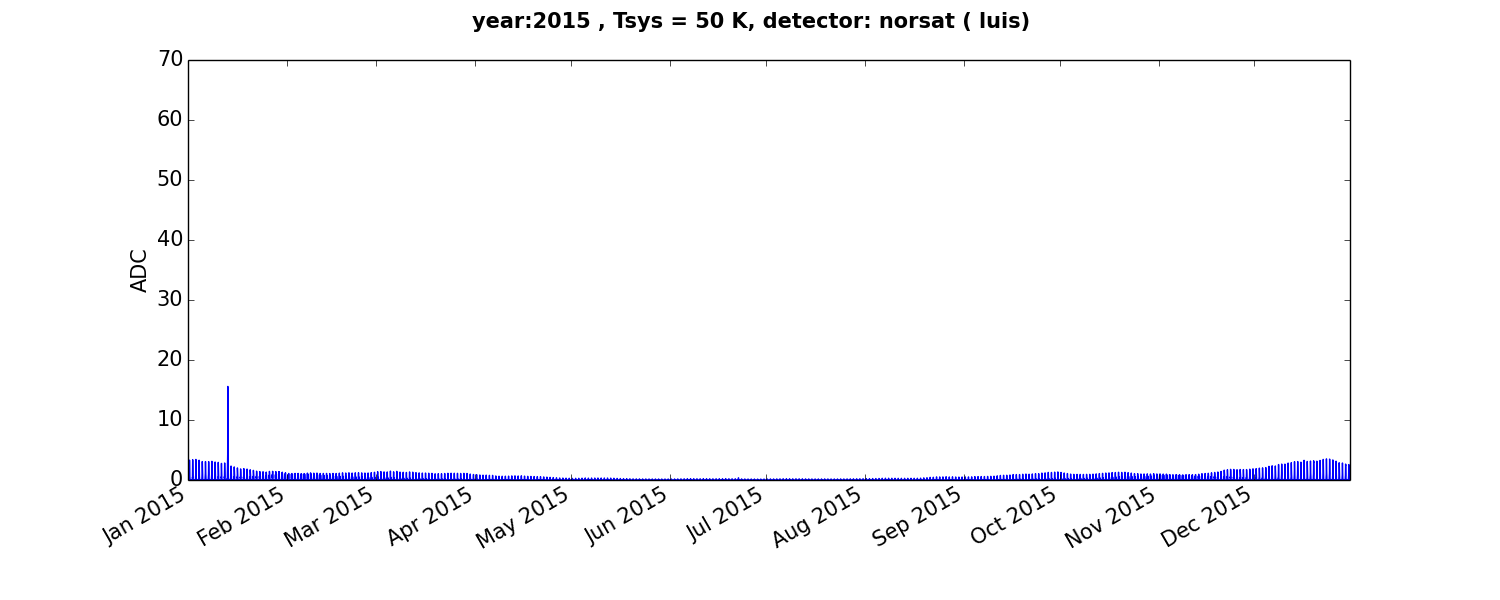
\includegraphics[width=0.7\linewidth]{year2015luis.png}}\\
  \caption{Left: quiet sun spectrum, Right: varying component spectrum}
  \label{fig:spectra}
\end{figure}



\section{Data description and baseline parameterization}
In this  section we attempt  to understand and parameterize  the radio
baseline.      We     will     separe    the     various     detectors
EASIER7/EASIER61/GIGADuck.  The first part  describes the basic cut we
apply,  the  second describes  the  baseline  parameterization we  can
obtain.  We analyse  the monitoring data recorded every  400 second at
the local  station.  The  data contains the  basic information  on the
radio  trace,  i.e.   the average  and  the  RMS.   But we  have  also
information  from the  Los Leones  weather station,  for  instance the
outside temperature and humidity.
\newpage
\subsection{a first look at the data and basic cuts}
We expect the radio baseline to vary because of different sources:
\begin{itemize}
\item a  variation of gain:  a variation of  gain is likely  to happen
  with temperature.
\item  the microwave flux:  if a  source strong  enough enters  in the
  field of view  of the antenna. This is what is  expected for the sun
  flux.
\item atmospheric effect:  this is also a variation  of the radio flux
  but it is  due to absorption of clouds, or an  increase of the field
  due to stormy conditions.
\end{itemize}
\subsubsection{overview}
We  show   the  raw   baseline  over  several   time  scales   in  the
figure~\ref{fig:scales}.
\begin{figure}[!ht]
  \centering
  \hspace*{-3ex}
  \subfigure{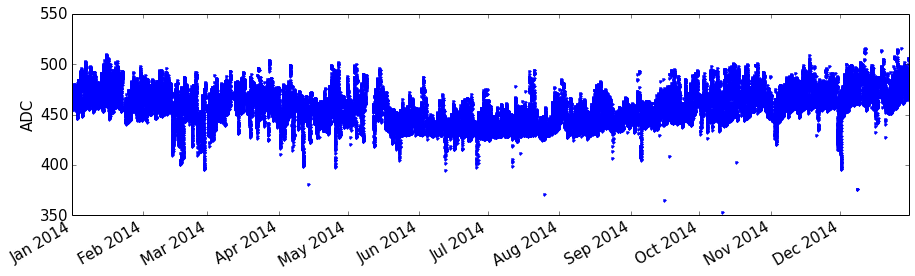
\includegraphics[width=0.9\linewidth]{oneyear.png}}\\
  \subfigure{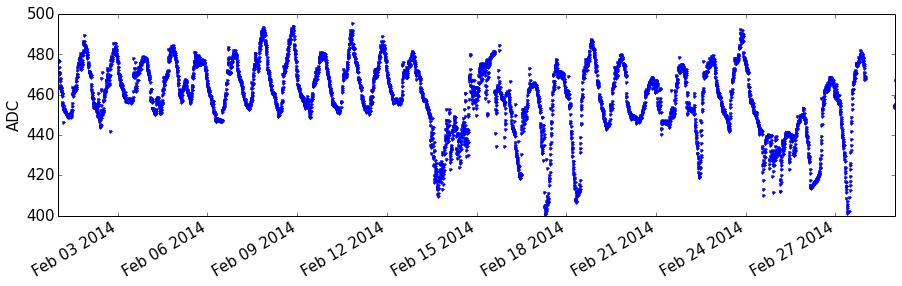
\includegraphics[width=0.9\linewidth]{onemonth.png}}\\
  \subfigure{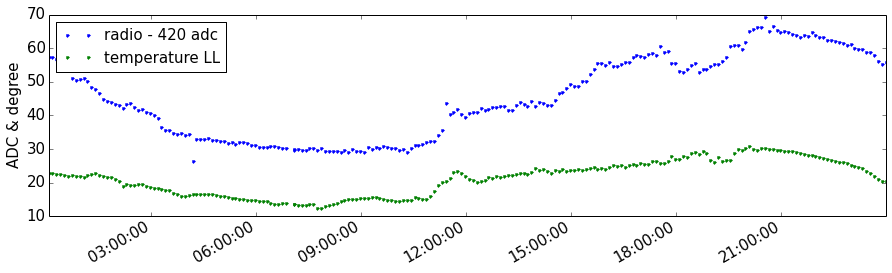
\includegraphics[width=0.9\linewidth]{oneday.png}}
  \caption{Left: quiet sun spectrum, Right: varying component spectrum}
  \label{fig:scales}
\end{figure}
We see  two main modulations,  a long term  variation one on  the year
long plot, and a daily modulation  on the month long plot. We can also
notice a  large decrease of the  baseline (i.e. increase  of the radio
power) for instance in the middle  of February. We will see later that
this can be related to rain. When there is no such rainy condition the
typical spread of the baseline  is around 40-50 ADC counts. However we
notice  clearly  on the  bottom  plot  of figure~\ref{fig:scales}  the
strong dependence with the outside temperature. \\ When we compare the
7     antennas     over      the     same     time     period     (see
figure~\ref{fig:allantennas}),  we notice the  structure has  the same
shape, but the amplitude of  the variations can be very different: for
instance stId332 has  variations of the order of  30-40 ADC counts and
stId 342 has variations of the order of 150 ADC counts)
\begin{figure}[!ht]
  \centering
  \hspace*{-3ex}
  \subfigure{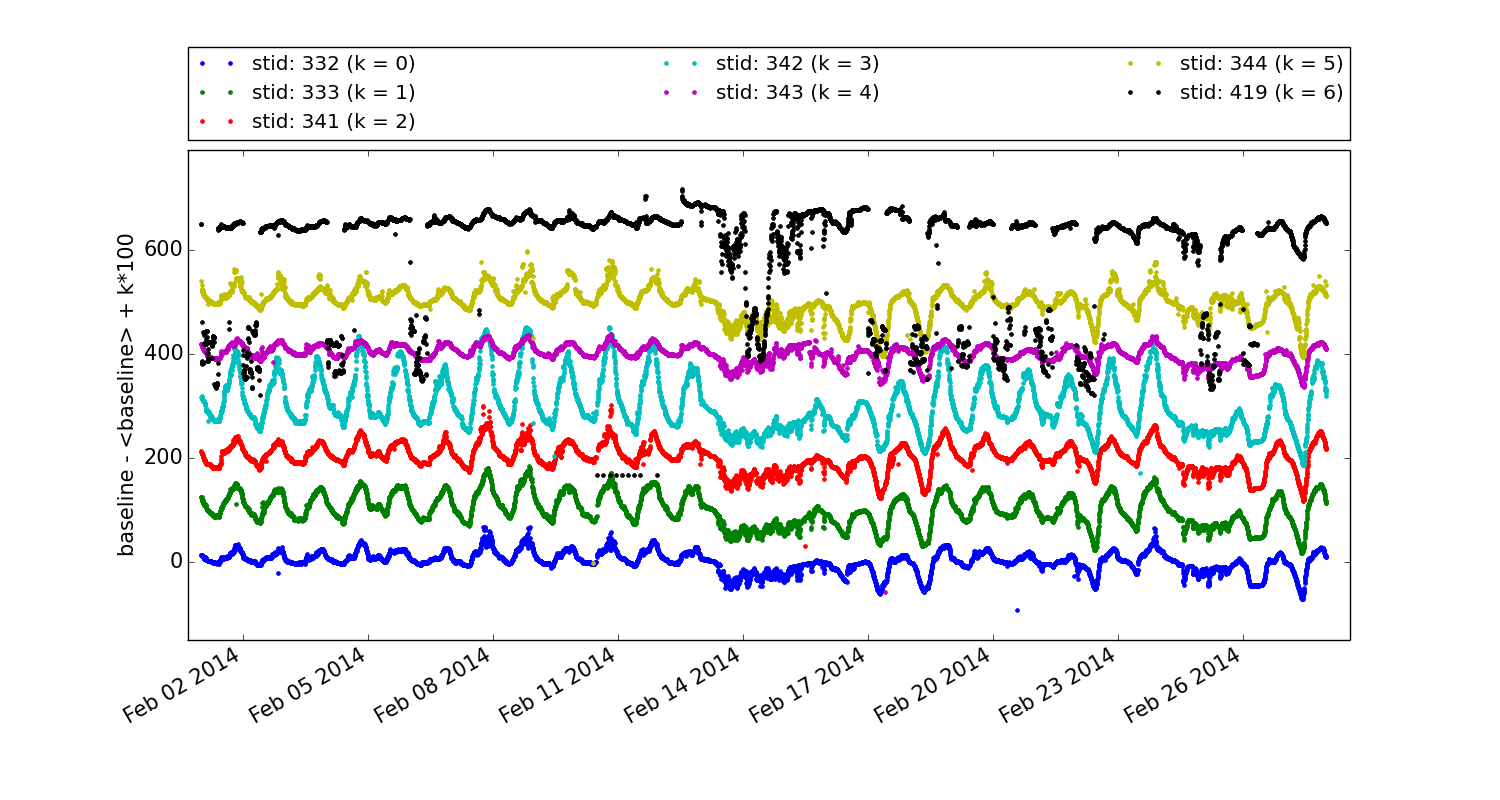
\includegraphics[width=0.9\linewidth]{allantennas.png}}
  \caption{}
  \label{fig:allantennas}
\end{figure}
In my opinion, these differences  are due to a different dependence of
the gain with the temperature.  The  gain itself is not related to the
system temperature, but it shows  that the 7 LNBf might have different
characteristics.
\subsubsection{cuts}
\paragraph{humidity}
We  have just  seen that  some periods  look very  different,  see for
instance around  February 15 in the  fig~\ref{fig:scales}. These large
baseline seem  to be related to the  rain.  Figure~\ref{fig:rain} show
the baseline  together with the humidity percentage  measured with Los
Leones weather station. It is  clear that a humidity larger than 60/70
\%  has a  strong  effect on  the  baseline.  This  effect  is more  a
threshold effect than a correlation:  when it rains we can't trust the
baseline.
\begin{figure}[!ht]
  \centering
  \hspace*{-3ex}
  \subfigure{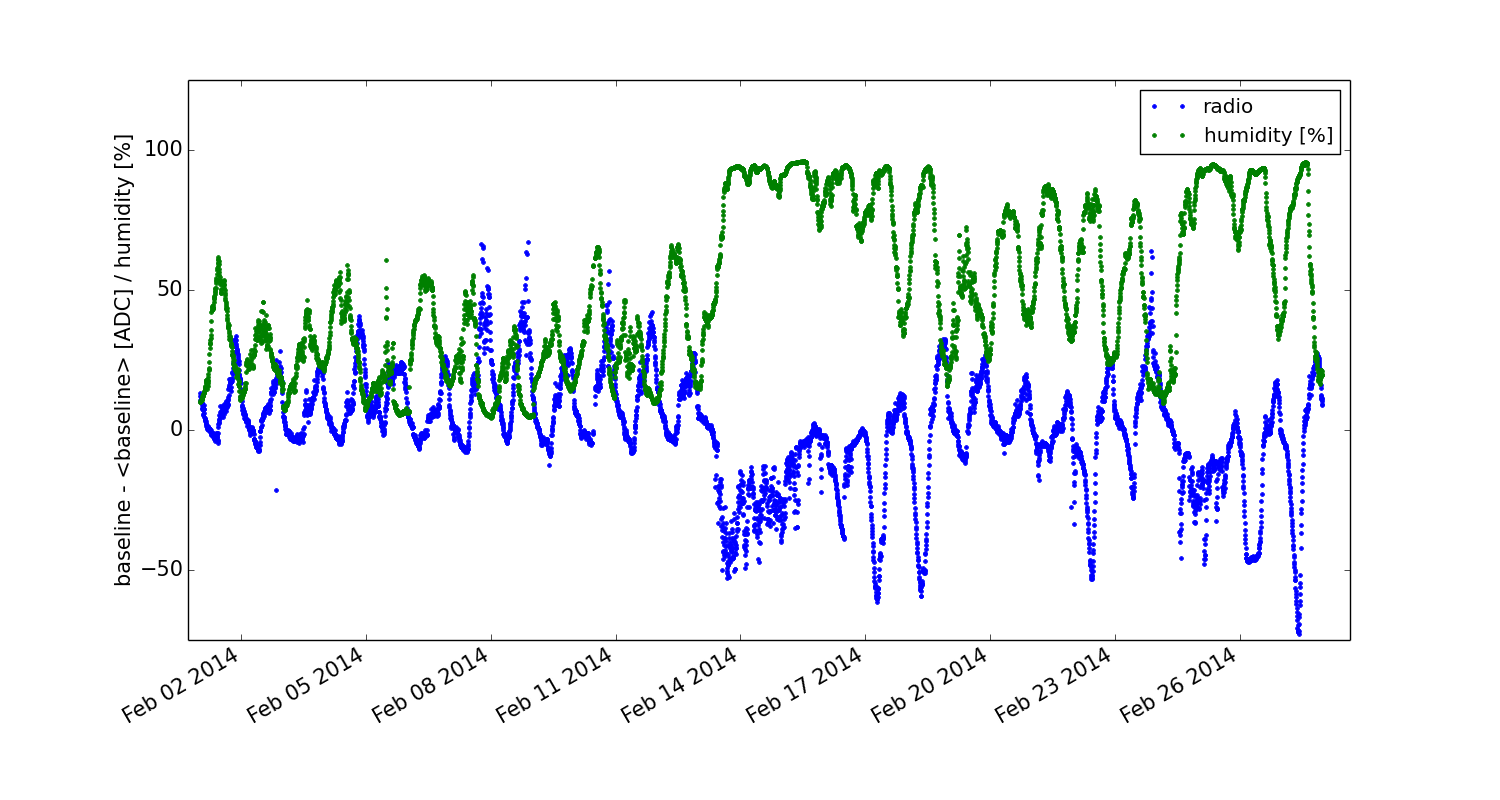
\includegraphics[width=0.9\linewidth]{radiohum.png}}
  \caption{}
  \label{fig:rain}
\end{figure}
In the following we require the humidity to be less than 50 \%.


\paragraph{sun/no sun periods}
The sun is expected to give a contribution to the baseline. We need to
exclude the period  when a significant signal is  expected in order to
keep  this effect.   The sun/no  sun periods  are determined  with the
expected signal calculated  above. We assume a temperature  of 50K for
the detector and  consider a signal above 5  ADC count as significant.
The figure~\ref{fig:sunnosun} is  an example of the split  of the data
in sun/no sun period (also after the humidity cut). 
\begin{figure}[!ht]
  \centering
  \hspace*{-3ex}
  \subfigure{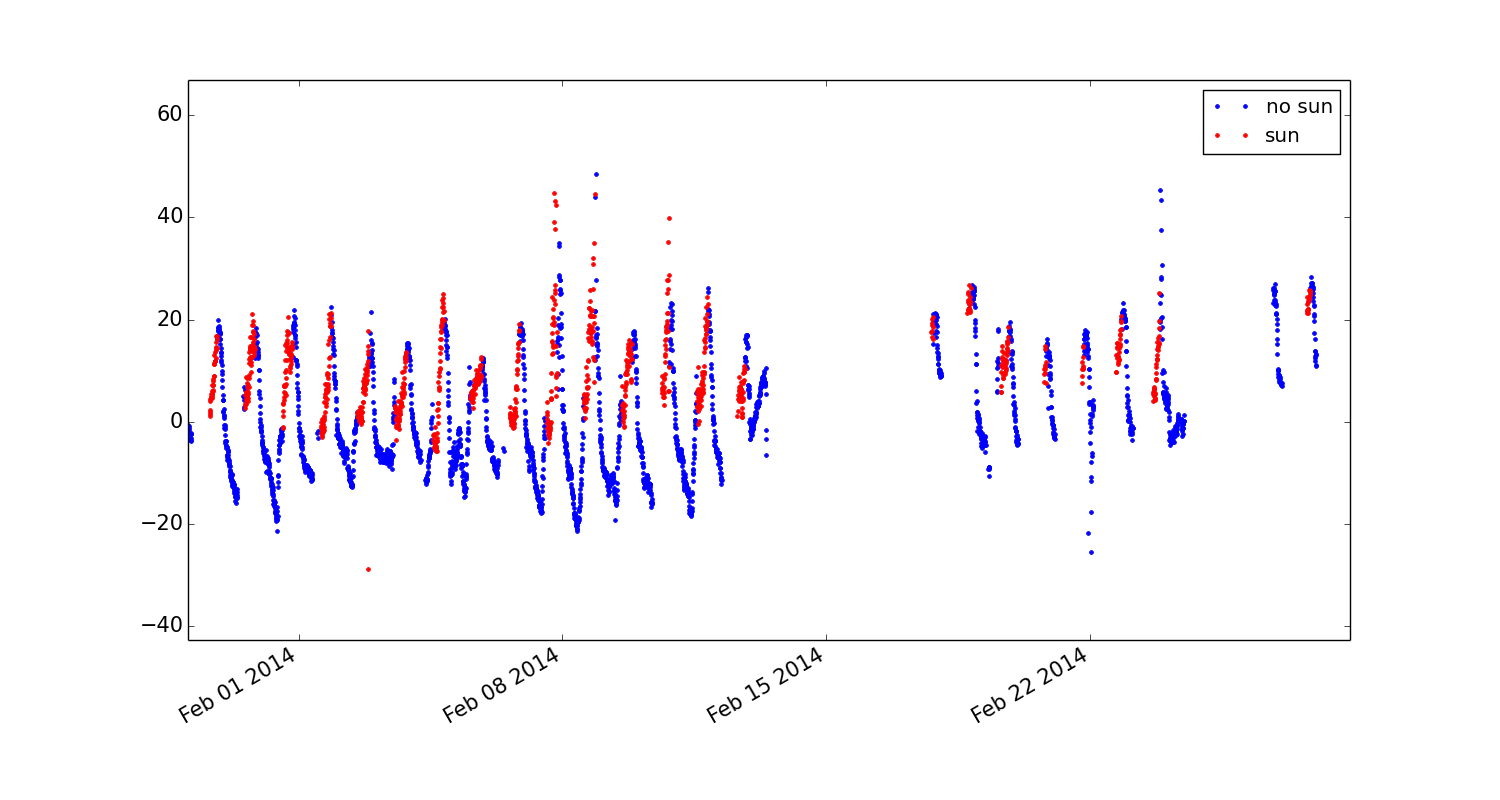
\includegraphics[width=0.49\linewidth]{sun_nosun.png}}
  \subfigure{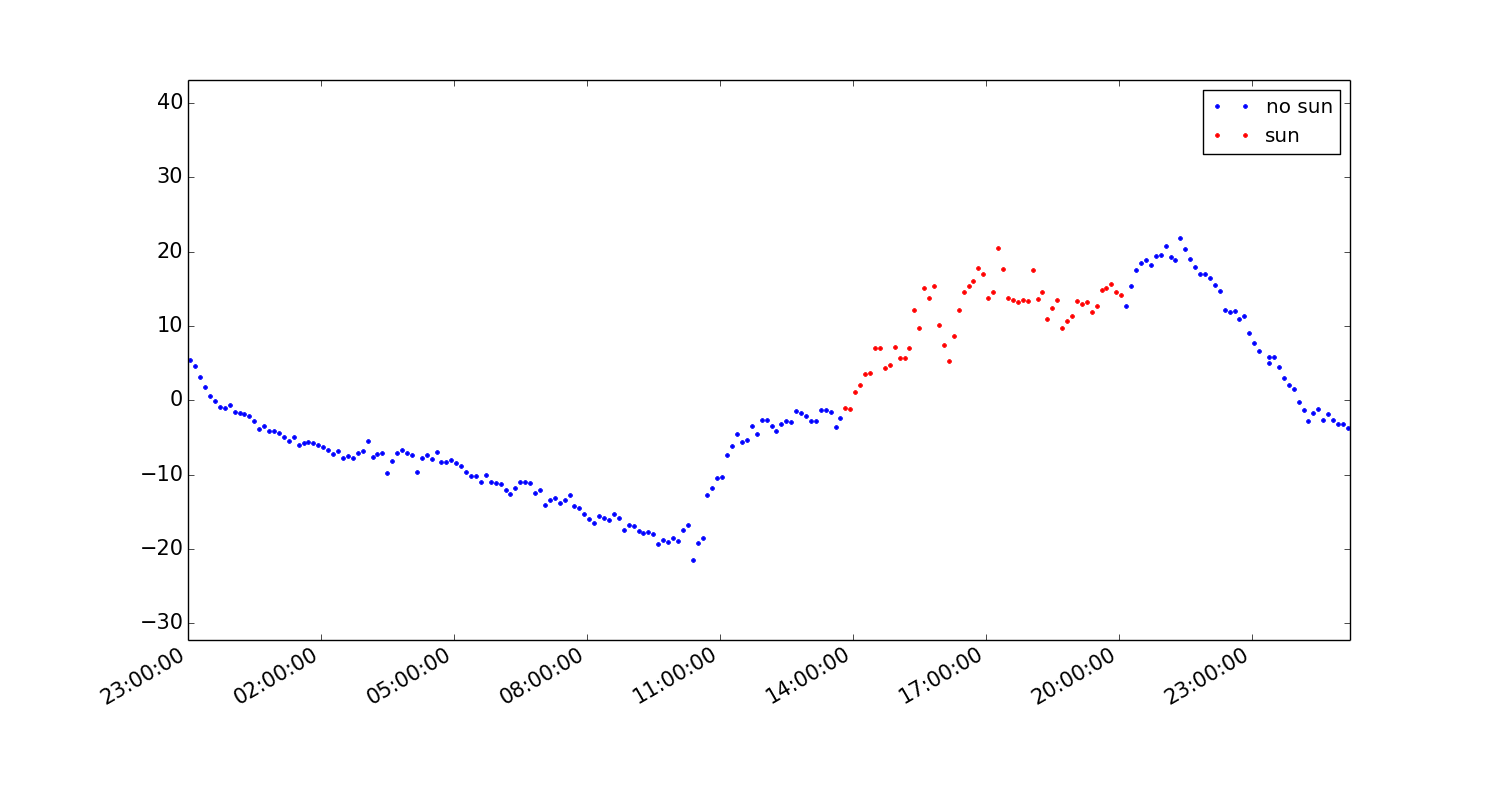
\includegraphics[width=0.49\linewidth]{sun_nosun2.png}}
  \caption{}
  \label{fig:sunnosun}
\end{figure}
\paragraph{long term variation}
We have seen that there is  a long term modulation of the baseline. To
remove this  dependence we filter  out the low frequencies  (below one
day). 

\subsection{Temperature parameterization}
The   radio   baseline   is   strongly  dependent   on   the   outside
temperature. The figures~\ref{fig:ybltemp}  shows the baseline against
the temperature for one year of data of the stations 332 and 342. This
can be explained  by a variation of the LNB  gain with the temperature
\cite{PStempnote}.   When we  perform  a linear  fit  and correct  the
baseline with this function, we  obtain a baseline distribution with a
spread of 5 to 16 ADC depending on the station.
\begin{figure}[!ht]
  \centering
  \hspace*{-3ex}
  \subfigure{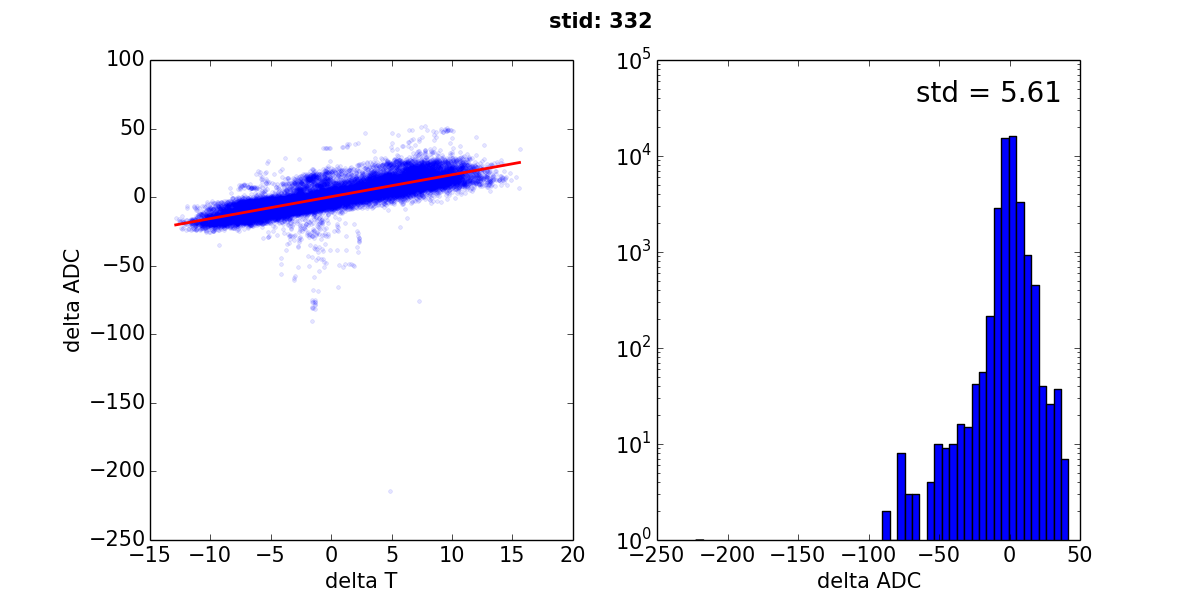
\includegraphics[width=0.9\linewidth]{yfit332.png}}\\
  \subfigure{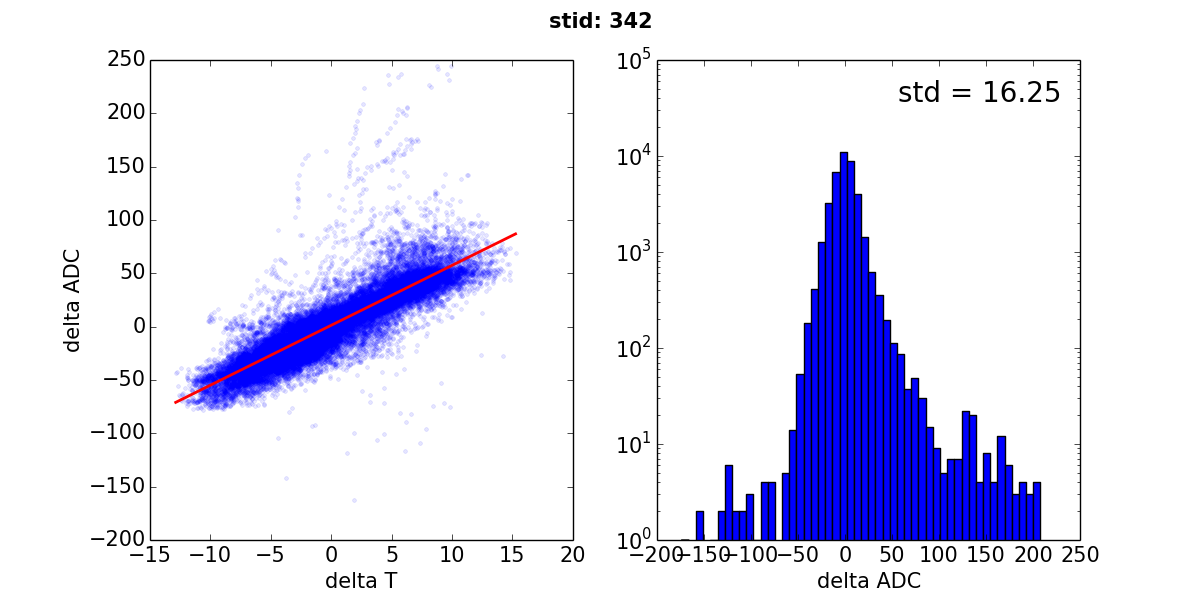
\includegraphics[width=0.9\linewidth]{yfit342.png}}
  \caption{}
  \label{fig:ybltemp}
\end{figure}

If we perform a daily fit  of the temperature dependence we can obtain
a   better   correction   of   the   baseline.    We   show   in   the
figure~\ref{fig:dbltemp} the  fits for  each day on  the left  and the
resulting corrected distribution on the right. 
\begin{figure}[!ht]
  \centering
  \hspace*{-3ex}
  \subfigure{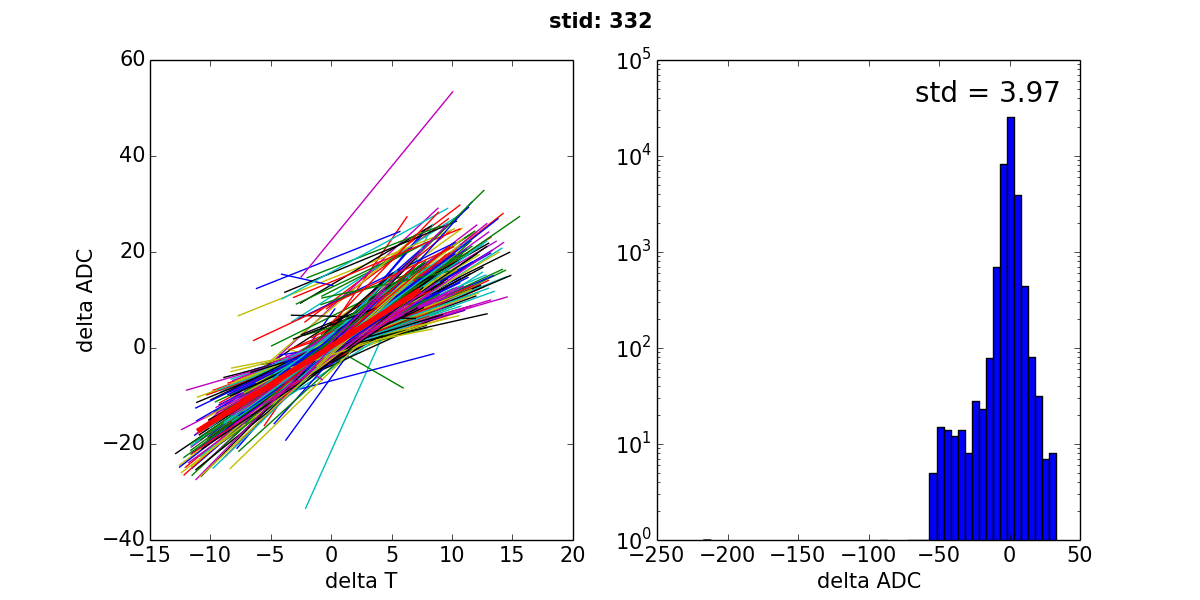
\includegraphics[width=0.9\linewidth]{dfit332.png}}\\
  \subfigure{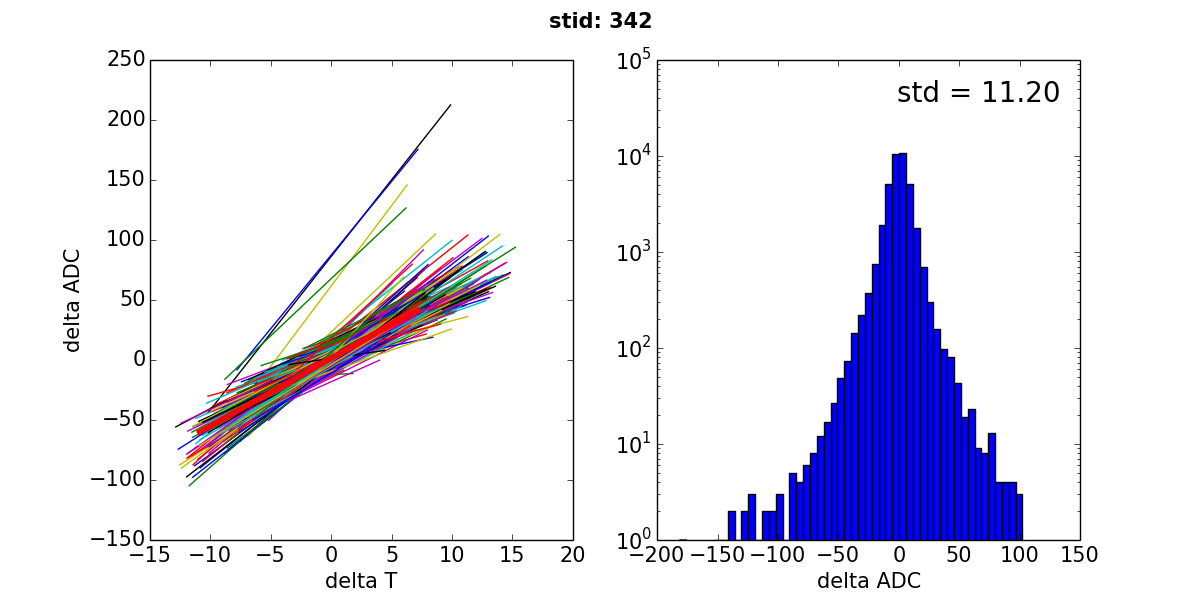
\includegraphics[width=0.9\linewidth]{dfit342.png}}
  \caption{}
  \label{fig:dbltemp}
\end{figure}
We  see that  the fits  can be  very different  depending on  the day,
meaning that other parameters are not accounted for. \\Furthermore, we
want  to be  able  to compare  a  \textit{non sun}  hypothesis with  a
\textit{sun}  hypothesis, so  we  need a  prediction  of the  baseline
during the time we expect the sun ( the sun signal is expected usually
between  11h00 and  16h00  in local  time,  i.e.  14h00  and 19h00  in
UTC).  In  the   figure~\ref{fig:prediction1}  we  show  the  baseline
comparison of  the baseline  between 14:00 and  19:00 for the  days we
don't expect the sun  signal. 
\begin{figure}[!ht]
  \centering
  \hspace*{-3ex}
  \subfigure{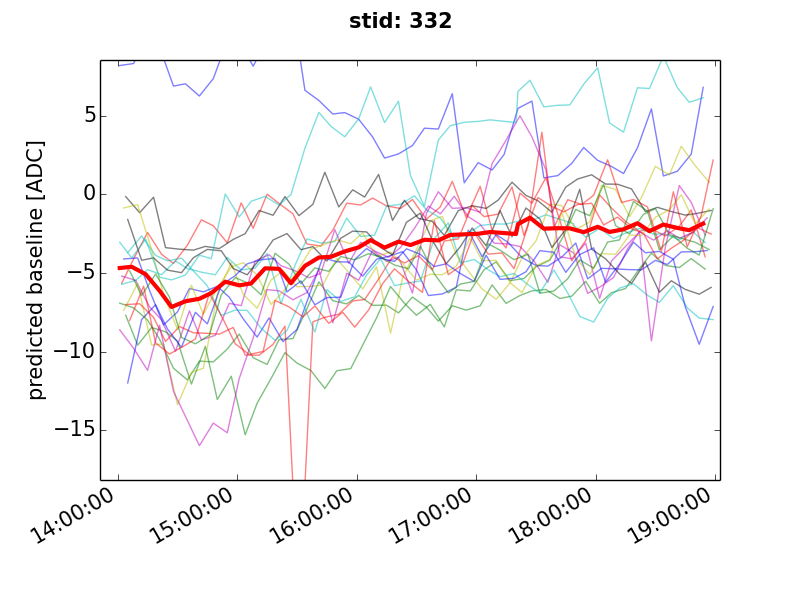
\includegraphics[width=0.32\linewidth]{yparam332.png}}
  \subfigure{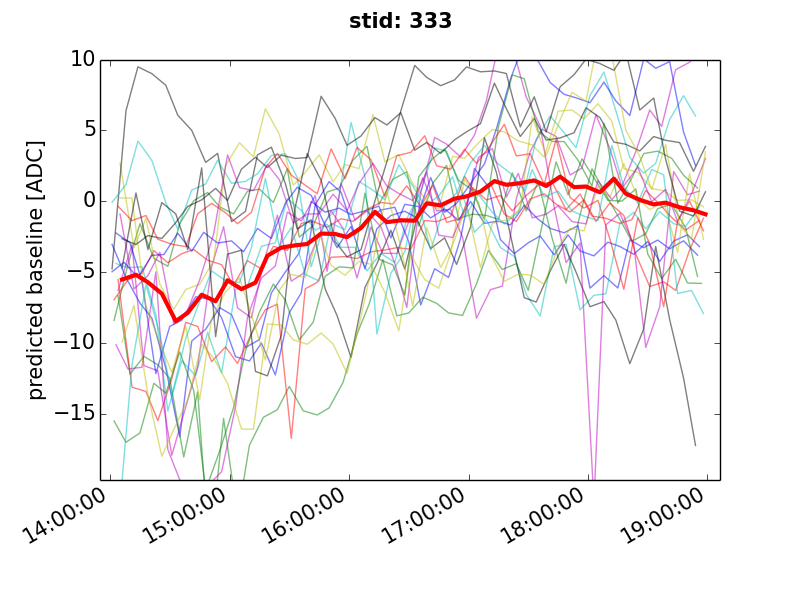
\includegraphics[width=0.32\linewidth]{yparam333.png}}
  \subfigure{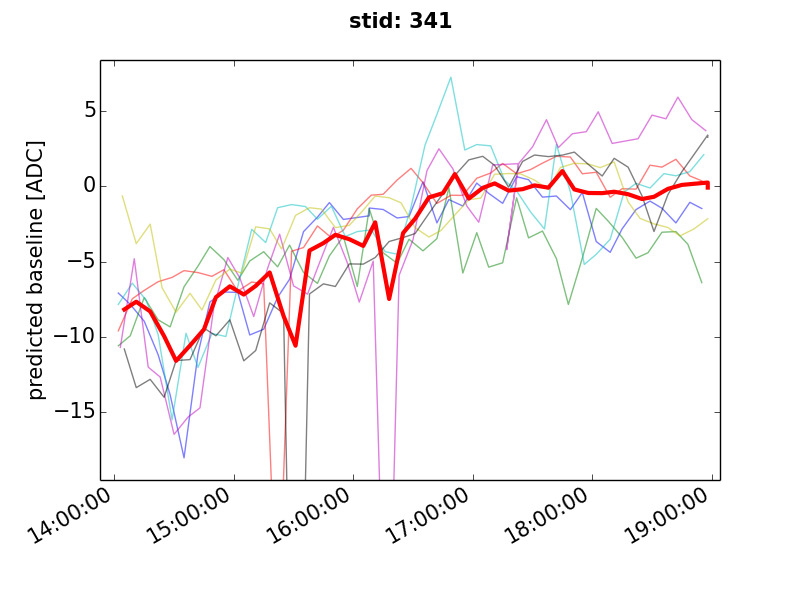
\includegraphics[width=0.32\linewidth]{yparam341.png}}\\
  \subfigure{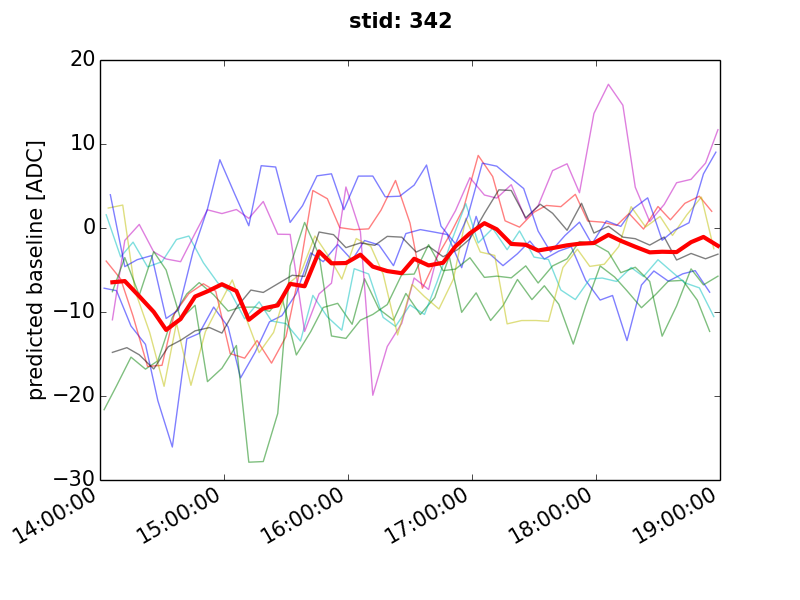
\includegraphics[width=0.32\linewidth]{yparam342.png}}
  \subfigure{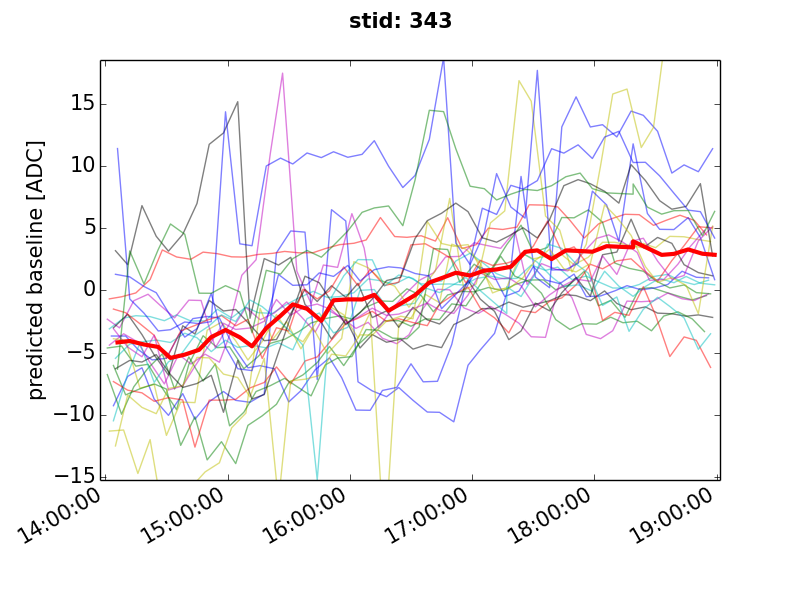
\includegraphics[width=0.32\linewidth]{yparam343.png}}
  \subfigure{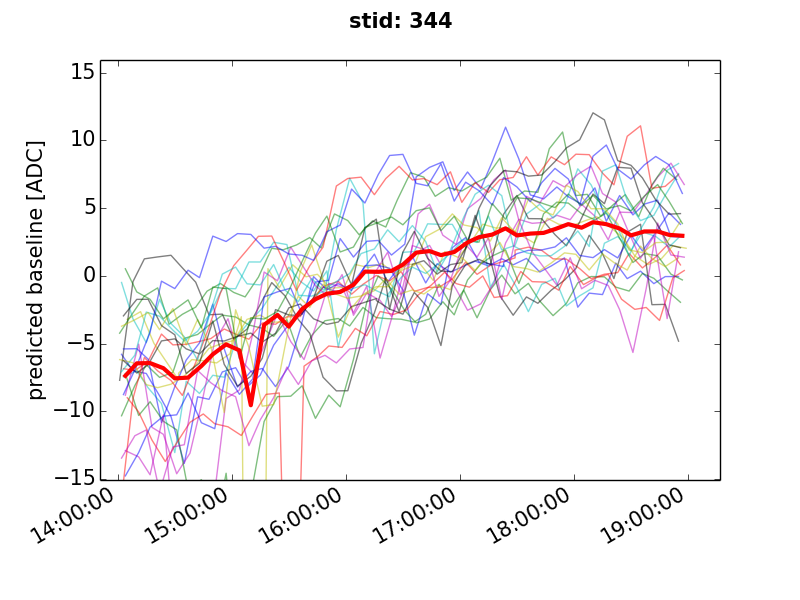
\includegraphics[width=0.32\linewidth]{yparam344.png}}
  \caption{baseline prediction with the temperature fit over a year}
  \label{fig:prediction1}
\end{figure}

\begin{figure}[!ht]
  \centering
  \hspace*{-3ex}
  \subfigure{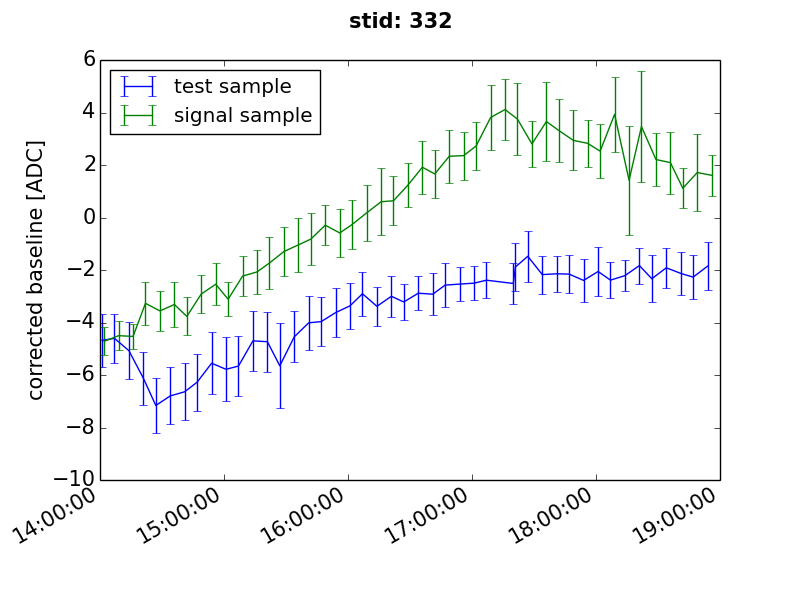
\includegraphics[width=0.32\linewidth]{yres332.png}}
  \subfigure{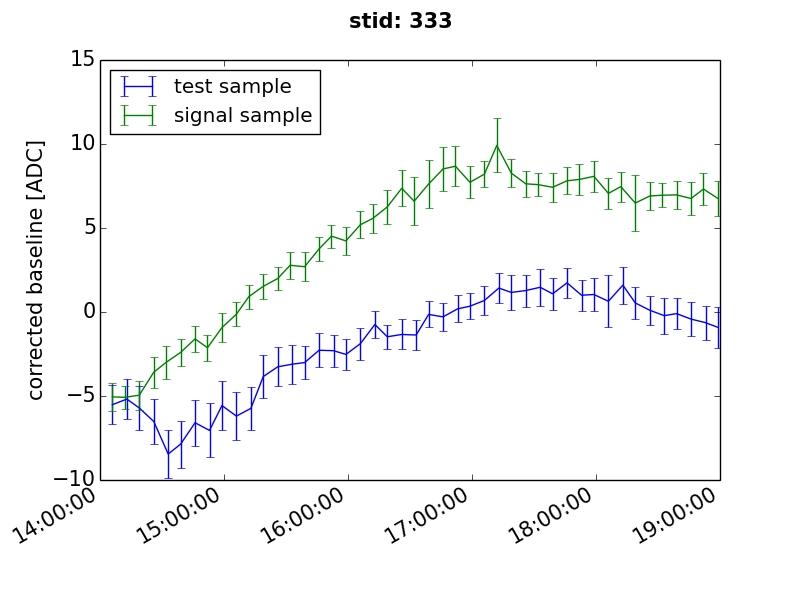
\includegraphics[width=0.32\linewidth]{yres333.png}}
  \subfigure{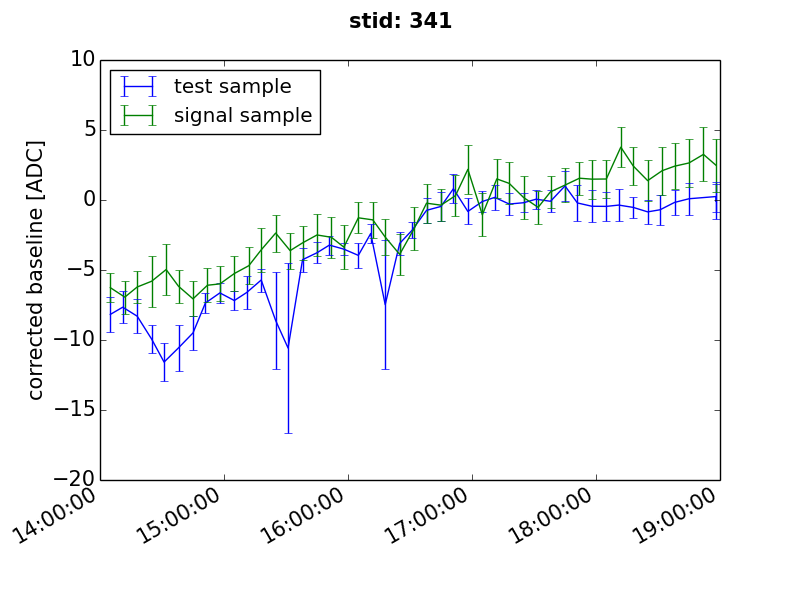
\includegraphics[width=0.32\linewidth]{yres341.png}}\\
  \subfigure{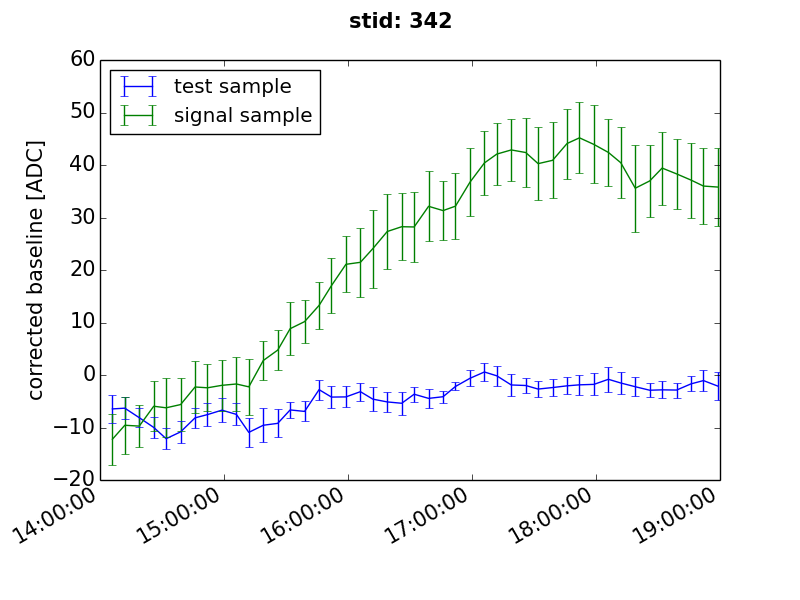
\includegraphics[width=0.32\linewidth]{yres342.png}}
  \subfigure{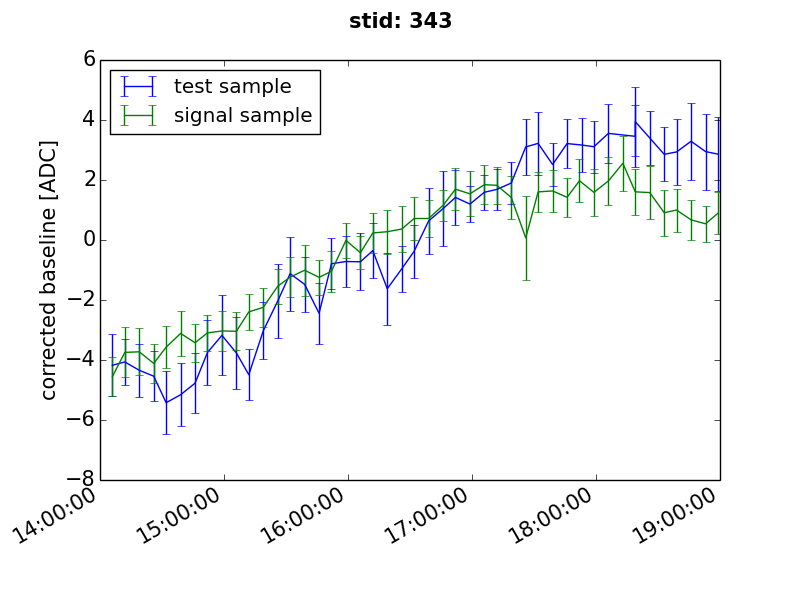
\includegraphics[width=0.32\linewidth]{yres343.png}}
  \subfigure{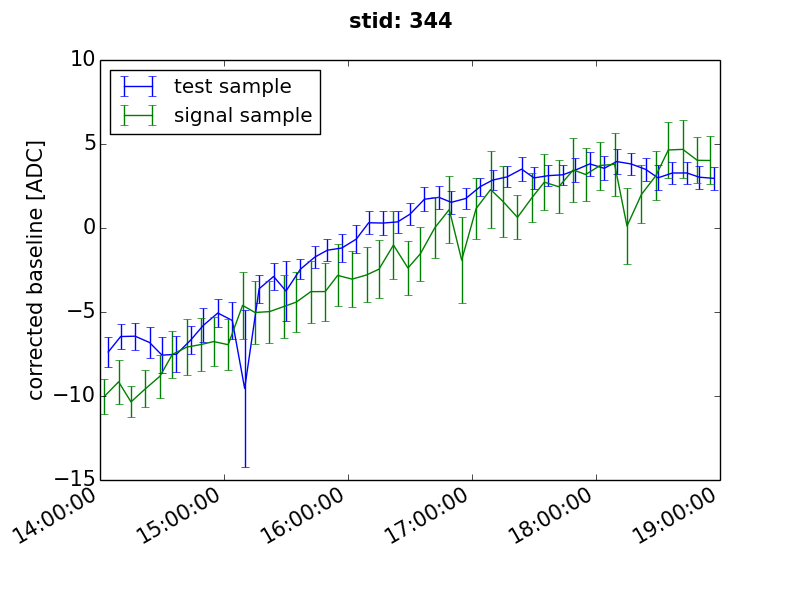
\includegraphics[width=0.32\linewidth]{yres344.png}}
  \caption{baseline prediction with the temperature fit over a year}
  \label{fig:prediction1}
\end{figure}

\newpage
\subsection{GIGADuck}
\begin{figure}[!ht]
  \centering
  \hspace*{-3ex}
  \subfigure{\includegraphics[width=0.9\linewidth]{GDnov.png}}
%%  \subfigure{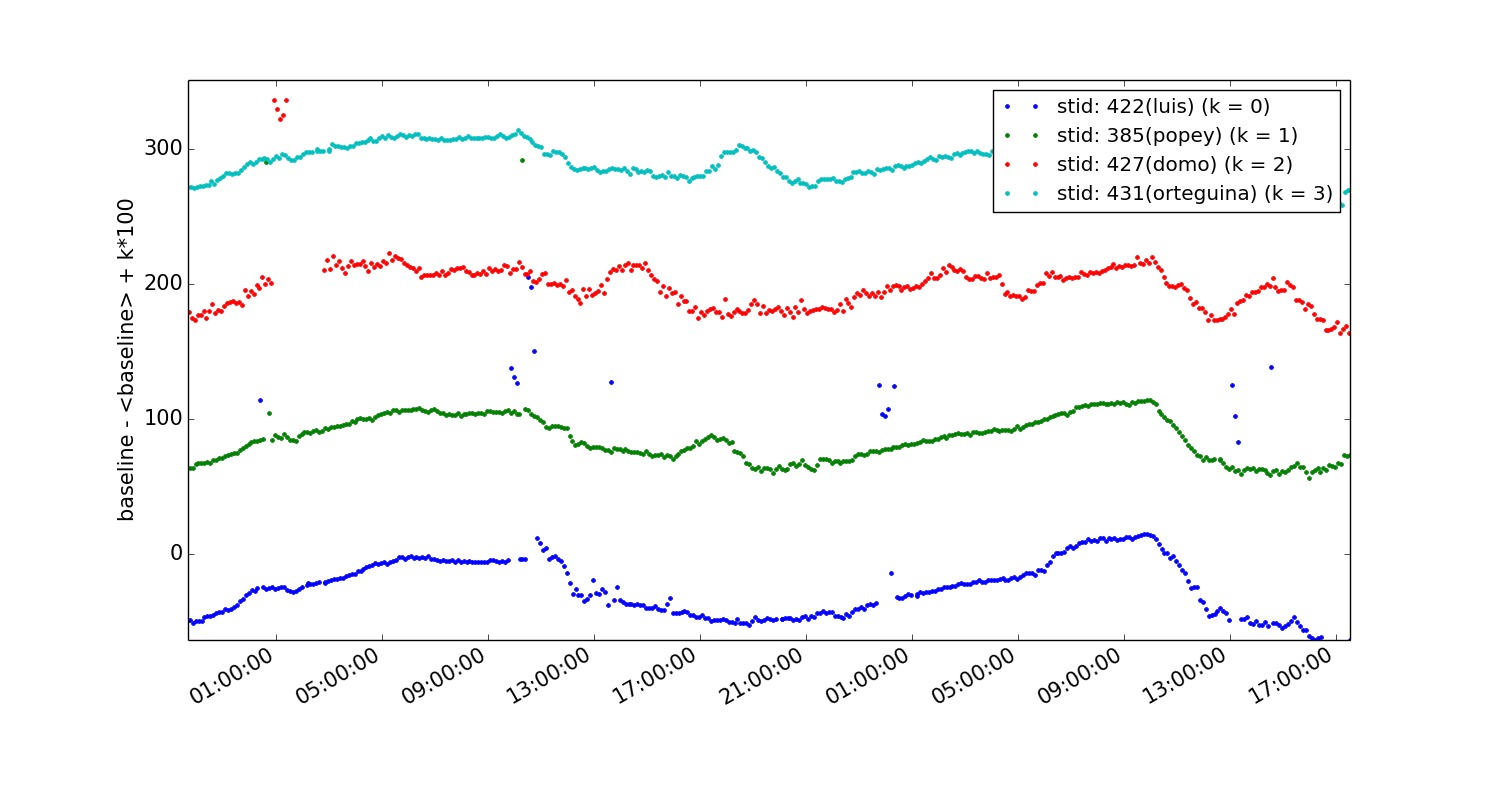
\includegraphics[width=0.49\linewidth]{GDjanzoom.png}}
  \caption{}
  \label{fig:gigaduck}
\end{figure}

\begin{figure}[!ht]
  \centering
  \hspace*{-3ex}
  \subfigure{\includegraphics[width=0.9\linewidth]{GDblvstemp.png}}
%%  \subfigure{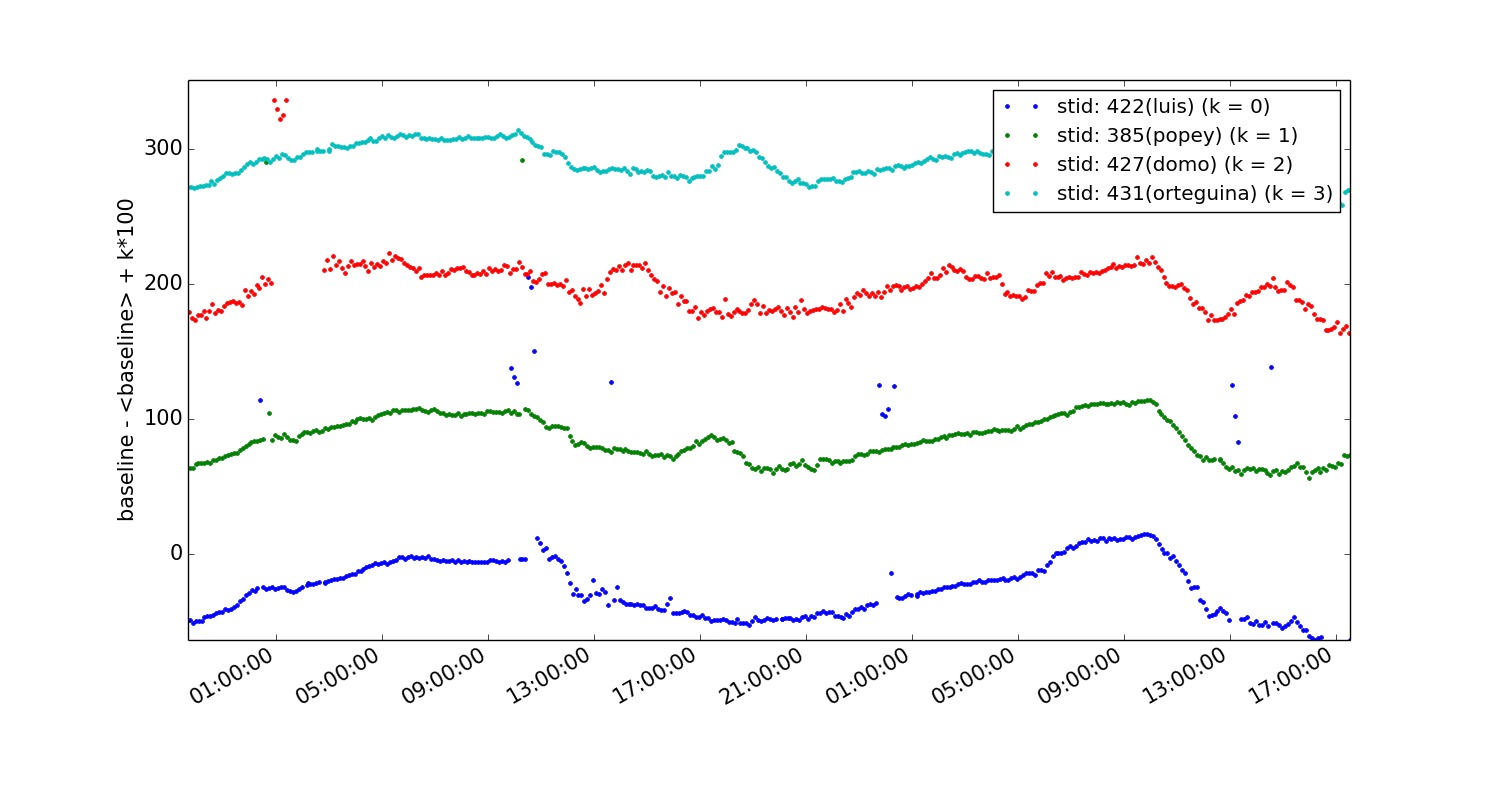
\includegraphics[width=0.49\linewidth]{GDjanzoom.png}}
  \caption{}
  \label{fig:gigaduck}
\end{figure}

\addcontentsline{toc}{chapter}{Bibliography}                                 
\bibliographystyle{atlasnote}
\bibliography{systemtemp}
%% \newpage
%% \begin{thebibliography}{9}
%% \bibitem{gorham}P. W. Gorham et al., Phys. Rev. D 78, 032007 (2008).
%%   [arXiv:0705.2589 [astro-ph]]
%% \bibitem{augerpolar} The Pierre Auger Collaboration, Phys. Rev. D 89, 052002 (2014)
%% \bibitem{crome}
%% \end{thebibliography}

\end{document}
